\documentclass[]{article}
\usepackage{indentfirst}
\usepackage{amsmath}
\usepackage{geometry}
\usepackage{amsthm}
\usepackage{amssymb}
\usepackage{graphicx}
\usepackage{float}
\usepackage{setspace}
\usepackage{booktabs}
\usepackage[colorlinks,linkcolor=blue]{hyperref}

\geometry{letterpaper,scale=0.7}
\linespread{2}
%opening
\title{Reconstruct Population Dynamics of White Tailed Deer (\textit{Odocoileus virginianus}) under Intensive Culling in Suburban Area, Chicago, IL}
\author{Yunyi SHEN\\
Submitted to F \& WE 875}
\begin{document}

\maketitle

\begin{abstract}
	%\linespread{1.05}
	%\renewcommand{\baselinestretch}{1.5}
	We did active culling to control white tailed deer (\textit{Odocoileus virginianus}) population in Chicago's sub urban area from 1992 to current. From age-at-harvest data we reconstructed the population size under intensive harvest from 1992-2006 using Bayesian reconstruction model we developed. Posterior expectation estimation suggest that population was controlled and stay stable to average 161 (sd=17) female between 1996 and 2006. Regression of vital rates with population size suggest there is a weak negative density dependency on fecundity older than fawn and no density dependency on survival.
\end{abstract}

\section{Introduction}
White tailed deer (\textit{Odocoileus virginianus}) is one of the most important game species in north America. However, over abundance of this species also cause problems, including over grazing one landscape, conflict with human and spread diseases like Crown Waste Disease. In suburban area, rapid growth of deer population increased the probability of human-deer conflict. In Chicago suburban area, increasing deer density promote concern of deer-vehicle collision (Etter et al. 2000 Witham \& Jones 1992). In 1992, 2 human were killed and 145 injured due to deer-vehicle collision (Etter 2002). Over growth of deer population also raise public health concern of zoonoses in this area (Miller 2001). 

%Harvesting was used as control method before in Chicago area, % talk about it

Researchers and Officials from Illinois Department of Natural Resources started to try intensive culling as population control method in Cook and DuPage Counties, Illinois (Complex 1) from 1992 to current. Reconstruction of population dynamic is needed to evaluate this method and its outcome.

Various method for reconstruction populations using multiple data sources were proposed recently (e.g. Iijima et al. 2013, Weldon et al. 2013). Bayesian method is one of the most promising approach. Stochastic matrix projection model is one of the most famous projection models for population with age structure (Leslie 1945). Bayesian framework of reconstruction allow us to fuse multiple data sources with different quality. Here we proposed and tested a Bayesian framework reconstruction modified from Wheldon et al. 2013 in order to understand the population's dynamic under culling. 

\section{Method}
\subsection{Study Area and Environment}
The study area encompassed 334,934 ha in the western suburbs of the greater Chicago metropolitan area, in Cook and DuPage Counties, Illinois. Land cover was dominated by urban/developed land (57.5\%) and associated urban grassland (14\%).  Other cover types included forested/woodland (14.2\%), cropland (4.9\%), rural grassland (4.1\%), wetland (3.3\%), open waters (1.8\%), and barren/exposed land (0.2\%; Illinois Department of Natural Resources 1996).

Population of study occupied complex 1 included Argonne National Laboratory (ANL), Waterfall Glen (WFG) and Woodridge (WDG) forest preserves located in southeast DuPage County, and Black Partridge forest preserve (directly adjacent to Woodridge) located in southwest Cook County, Illinois. Habitat area of this complex remained constant through culling years.
\subsection{Intensive Culling}
Prior to 1992, no deer were legally harvested in Complex 1. Culling in Complex 1 started in WFG in 1992. In 1993 and 1994, we culled deer from WFG and WDG, and beginning in 1995 we culled deer from ANL and all other forest preserve in Complex 1. Deers were culled during October–April by sharpshooting, and capture and euthanasia as described by Etter (2001) and DeNicola et al. (2008).  Antlerless deer were prioritized, but deer were culled on a first opportunity basis.

\subsection{Data Collection and Initial Estimation}
Culled deers were aged into 8 age classes and recorded from 1992 to 2006. Initial estimation and their uncertainty which also serves as prior mean of vital rates and used to determine hyperparameters came from previous study in the same area (Etter 2001). Initial estimation of harvest rate was the ratio between previous reconstruction study in the same population and total culling count, while we assume harvest rate of fawns was half of harvest rate of adult since the protocol of culling was strongly biased toward non-fawns. 

\subsection{Bayesian Reconstruction of Population Dynamics under Culling}
\subsubsection{Notations and Parameterization}
Parameters of interest are time and age specific fecundity and survival, as well as harvest rate and population size of female deers in study area. We later on use $C_{a,t}$ for culling counts at age $a$ and time $t$, $s_{a,t}$ for survival, $f_{a,t}$ for fecundity, $H_{a,t}$ harvest rate, $X_{a,t}$ for latent living population size after culling and $M$ for the matrix projection model. Bold form of value is the the corresponding age vector (e.g. $\mathbf{C}_{t}=(C_{1,t},C_{2,t}...)$). Underline of certain parameters means the best estimation and data we have currently that will be used in the model. (see Fig.\ref{Fig.Bayes}) 

\subsubsection{Projection Model for Culling Dynamics}
We assume a time inhomogeneous stochastic proportional harvest. Further, harvest rate of fawns (age 0.5) is assumed to be different from yearling and adults (age $>0.5$). We used a diagonal harvest matrix $\mathbf{H}_{t}$ to model the harvest in the projection to seperate harvest and other mortality. Growth of living individuals are projected using standard stochastic Leslie matrix model (Leslie 1945). Leslie matrix contains $s_{a,t}$ and $f_{a,t}$ was noted by $\mathbf{L}_{t}$. Since harvest happened after reproduction, we left multiply the harvest matrix. Vital rates' distribution as described in the prior part of the Bayesian framework.

Formally the projection model of harvest count vector $\mathbf{C}_{t}$ is given by:
\begin{equation}
\label{proj}
\mathbf{C}_{t+1}=\mathbf{H}_{t+1}\mathbf{L}_{t+1}(\mathbf{H}_{t}^{-1}-\mathbf{I})\mathbf{C}_{t}
\end{equation}  

In which $I$ is identity matrix. Note that $(\mathbf{H}_{t}^{-1}-\mathbf{I})\mathbf{C}_{t}$ solves the living individual after culling that undergone reproduction at time $t+1$. Also note that baseline year should be trait differently since there is no $L_{0}$ needed. A graphical illustration of the dynamics is given in Fig.\ref{Fig.LHD}.

\begin{figure}[htbp] % life history graph
	\centering
	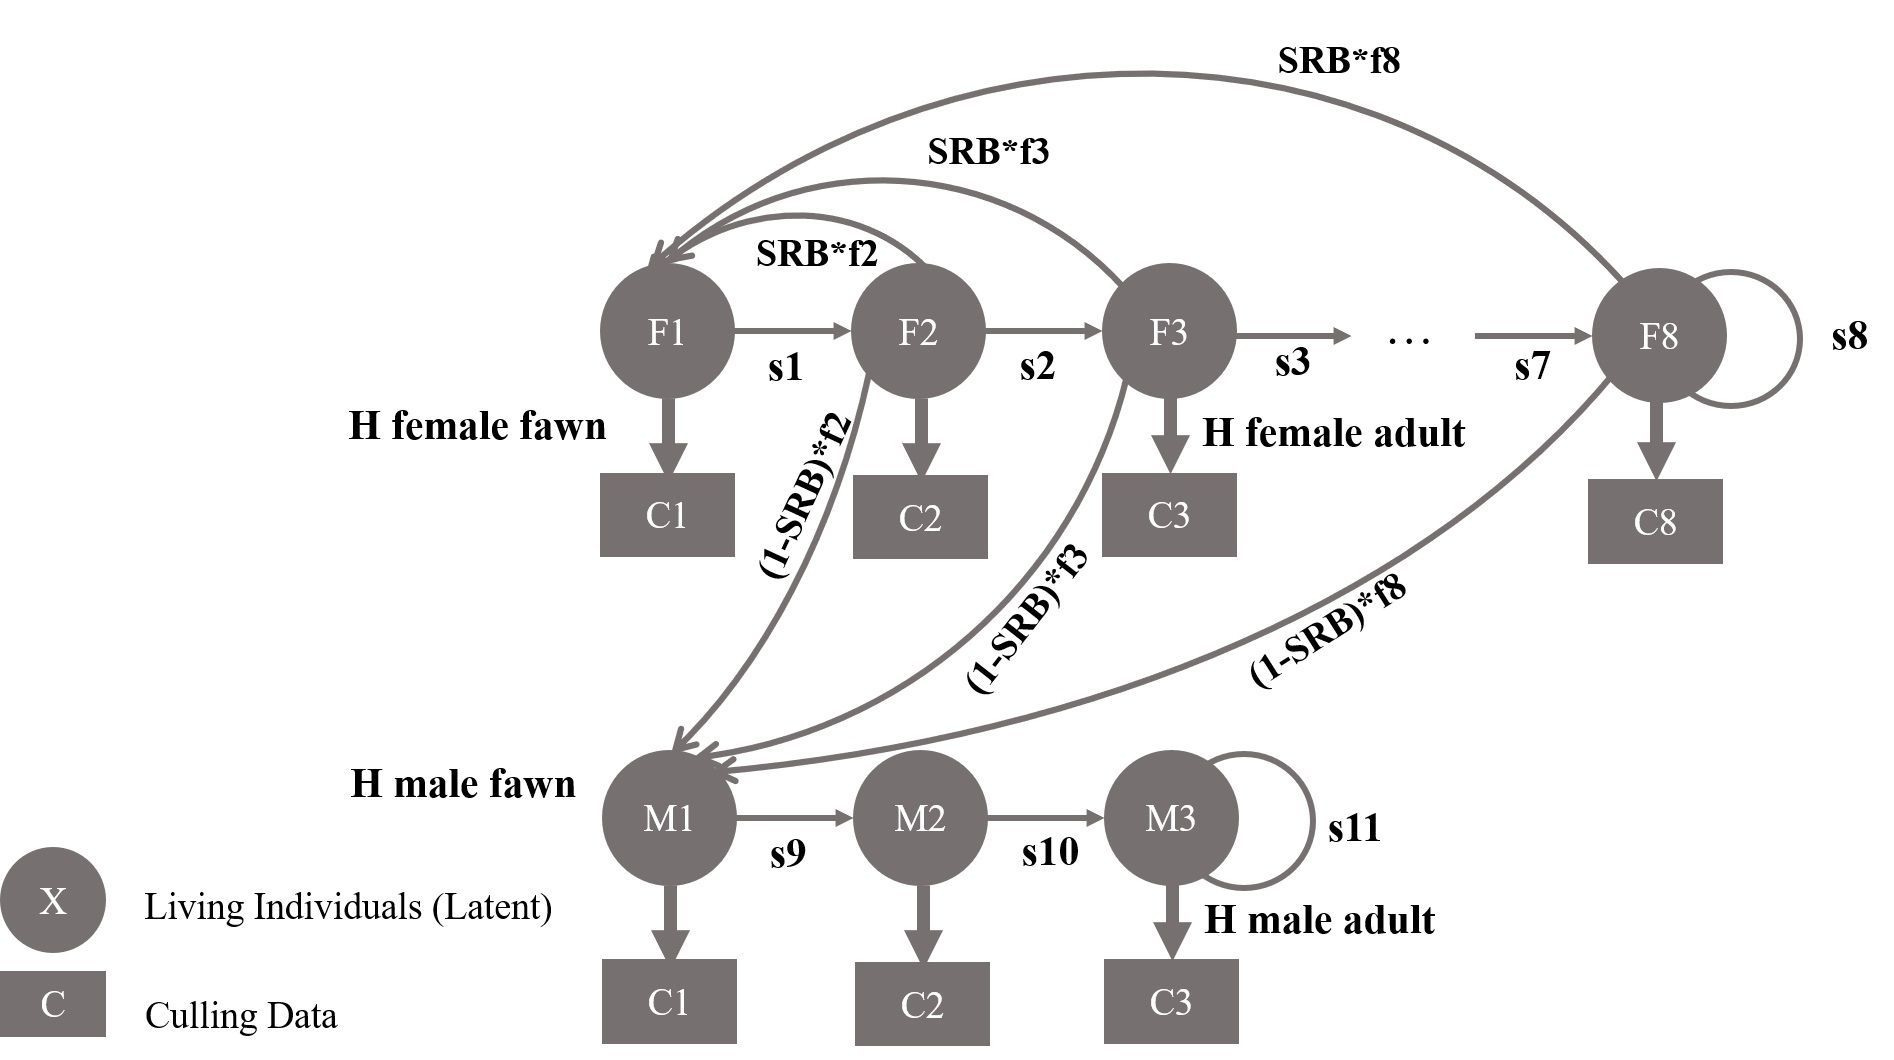
\includegraphics[width=0.8\linewidth]{figs/LHD.jpg}
	\caption{Projection Model used in Bayesian Framework for Culling Dynamics}
	\label{Fig.LHD}
\end{figure}

\subsubsection{Bayesian Reconstruction}
We generally followed Wheldon et al. 2013's Bayesian reconstruction framework, except we had a new set of parameters regarding the harvest rate and did not have migration. Projection model used in our study was described by eqn.\ref{proj}. Reconstruction is equivalent of estimating vital rates $s$, $f$, $H$ and population population counts $X$. We used the same 4 level setting to count for uncertainty of initial estimation (Fig.\ref{Fig.Bayes4level})

\begin{figure}[htbp] % 4 level graph
	\centering
	\includegraphics[width=0.8\linewidth]{figs/Bayesian_model_4level.jpg}
	\caption{Prior and Likelihood Part of the Bayesian Reconstruction Framework}
	\label{Fig.Bayes4level}
\end{figure}

Relationship between data and parameters were shown in Fig.\ref{Fig.Bayes}. Note that $\alpha_{v}$ and $\beta_{v}$ $v\in\{s,f,H,C\}$ are hyperparameters which encode the prior knowledge we have for the uncertainty of certain vital rate or culling count. Initial estimations of survival (logit transformed), fecundity (log transformed) and harvest rate (logit transformed) were used as corresponding transformed prior mean of the normal distribution whose $\sigma$ was invGamma distributed with parameter $\alpha_{v}$ and $\beta_{v}$ $v\in\{s,f,H,C\}$. Culling count served in the likelihood part of the model, log transformed model predicted culling count $C$ serves as mean of the likelihood function while variance $\sigma$ came from invGamma distribution similar to before. 

\begin{figure}[htbp] % bayes graph
	\centering
	\includegraphics[width=0.8\linewidth]{figs/Bayesian_model.jpg}
	\caption{Relationship between Various Data and Parameters in the Bayesian Reconstruction Model for Culling Dynamics}
	\label{Fig.Bayes}
\end{figure}





\subsubsection{Determining the Hyperparameters}
Determination of hyperparameters $\alpha$ and $\beta$ for vital rates except for harvest rate were based on previous study's error estimation, use the same method in Wheldon et al. 2013, but more conservative. Harvest rate's hyperparameter were set to be enough conservative that has .95 quantile $>2$ ($\alpha=1$,$\beta=.1$). Detail hyperparameter setting is shown in Table.\ref{tab:hyper}
\begin{table}[htbp] % model checking table
	\centering
	\caption{\label{tab:hyper}Hyperparameter Setting in This Study}
	\begin{tabular}{ccccc}
		\toprule
		&Survival&Fecundity&Harvest&Count \\
		\midrule
		$\alpha$&1&1&1&1\\
		$\beta$ &.1&.01&.1&.01\\
		\bottomrule
	\end{tabular}
\end{table}

\subsubsection{Estimation}
We draw samples from posterior distribution using Markov chain Monte Carlo (MCMC) method (Metropolis et al. 1953, Hastings 1970) and diagnose using R package \texttt{coda} (Plummer et al. 2006). The algorithm generally followed Wheldon et al. 2013. We updated variance ($\sigma^{v}$s) from conjugated full conditional distributions as proposed density in Metropolis-Hastings algorithm. Other vital rates including culling rate were updated using Metropolis-Hastings steps and a symmetric normal proposal. Algorithm was tuned by hand to achieve a reasonable acceptance rate. Follow Wheldon et al., "iteration" was defined as one complete sweep through all age- and time-specific parameters and variance parameters.


\subsubsection{Living Individuals}

After we reconstruct the culling dynamics $\mathbf{C}_{t}$ and harvest rate $\mathbf{H}_{t}$, we solve the living individual after culling $\mathbf{X}_{t}$ using eqn. \ref{eqn.living} 

\begin{equation}
\label{eqn.living}
\mathbf{X}_{t}=(\mathbf{H}_{t}^{-1}-\mathbf{I})\mathbf{C}_{t}
\end{equation}  


The model is implemented in R 3.5.3 (R core team 2019) modified from package \texttt{popReconstruct} (Weldon et al. 2013). Source code is available on \href{https://github.com/YunyiShen/DDLeslieReconstruct}{\texttt{GitHub}} under MIT license.

\section{Results}
\subsection{Data Collection}
Total 15 years of culling count was used in this study (1992-2006, 1992 as baseline). In 15 years total 3827 individuals were culled. Fecundity and survival estimation was homogeneous for all age $>1.5$, however we keep this. Average fecundity for adults is 1.86, yearling 1.53 and fawn 0.178. Mean survival rates are 0.85, 0.82 and 0.83 for fawn, yearling and adults respectively (Etter 2001). Mean harvest rate for the population is 0.5 (Etter et al. 2019 unpublished data).
\subsection{Model Checking}
We use 2 distinct model checking indexes, Absolute Difference (AD) defined as absolute value of difference between model predicted culling counts and real counts which evaluates precision of the model. Posterior Standard Deviation (PSD) defined as standard deviation of posterior distribution of model predicted culling which evaluated uncertainty of prediction.

\begin{table}[htbp] % model checking table
	\centering
	\caption{\label{tab:check}Model Checking Indexes for Reconstruction of Culling Data}
	\begin{tabular}{ccc}
		\toprule
		&Mean&Standard Error\\
		\midrule
		Absolute Difference&11.19 & 1.93\\
		Posterior Standard Deviation & 14.89 & 0.36\\
		\bottomrule
	\end{tabular}
\end{table}


\subsection{Living Individuals After Culling}
After reconstruct the culling dynamic, we solved the total living individuals' posterior distribution as described by eqn.\ref{eqn.living}. Results were shown in Fig.\ref{Fig.popsize}. After 1996, posterior mean showed the population was stabled around average 161 (sd=17) female individuals which achieved our goal of controlling the population. Harvest rate for fawns has mean of 0.26 and sd of 0.05, for other than fawns has mean of 0.53 and sd of 0.13. 
\begin{figure}[htbp] % popsize table
	\centering
	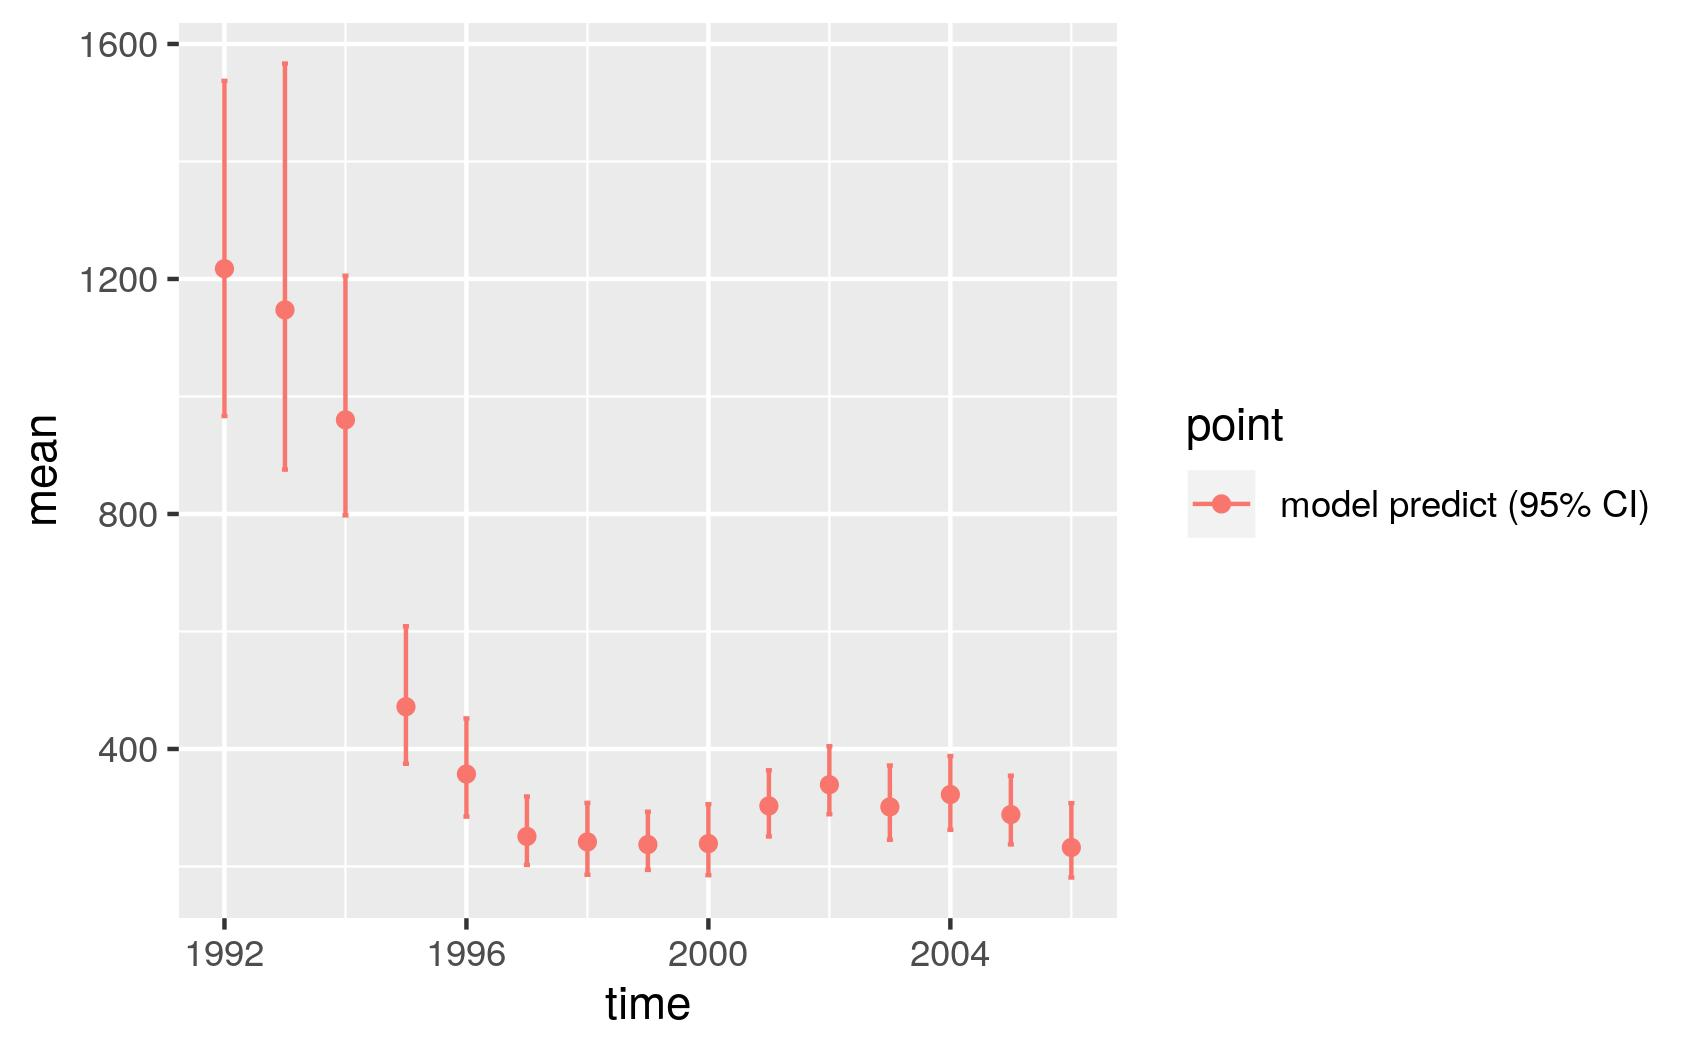
\includegraphics[width=0.8\linewidth]{figs/popsize.png}
	\caption{Reconstructed Population Size After Culling}
	\label{Fig.popsize}
\end{figure}

\subsection{Density Dependency of Vital Rates}
Density dependency is one of the key features controlling population growth (Ueno et al. 2010). To address whether there exist density dependency we did linear regression between vital rates and reconstruct living population size before reproduction (i.e. living individual counts after culling of the previous year). Results were summarized in Table.\ref{tab:DDvital}. Only fecundity rates of age after fawn show weak negative density dependency which agree with our expectation of deer biology. 

\begin{table}[htbp] % DD_fatal table
	\centering
	\caption{\label{tab:DDvital}Linear Regressions of Vital Rates and Population Size after Culling}
	\centering
	\begin{tabular}{lcccccccc}
		\toprule
		Age  &0.5&1.5&2.5&3.5&4.5&5.5&6.5&7.5\\
		\midrule
		\textbf{\textit{Fecundity}} & & * &* &* &* &* &* &* \\
		p-value & 0.0981&0.0231&0.037&0.0325&0.0366&0.0324&0.0411&0.0364\\
		adj $R^2$&0.1457&0.3076&0.2573&0.2714&0.2583&0.2716&0.2456&0.259\\
		$\beta$ &-1.13E-04&-0.000888&-0.00108&-0.0011&-0.00108&-0.0011&-0.00104&-0.00105\\
		SE $\beta$&6.30E-05&0.0003411&0.0004632&0.0004595&0.00046&0.000456&0.000458	&0.000448\\
		%\midrule
		\textbf{\textit{Survival}} & & & & & & & & \\
		p-value&0.0714&0.647&0.899&0.142&0.619&0.575&0.66&0.873\\
		adj $R^2$ &0.183 &0 &0 &0.1012 &0 &0 &0 &0\\
		$\beta$&-1.48E-05&-7.06E-06&1.04E-06&1.18E-05&-4.19E-06&8.23E-06&5.39E-06&-9.80E-07\\
		SE $\beta$ &7.46E-06&1.51E-05&8.07E-06&7.53E-06&8.22E-06&1.43E-05&1.17E-05&6.05E-06\\
		
		\bottomrule
		 *:$p<0.05$&
	\end{tabular}
\end{table}


\section{Discussion}
By conducting intensive culling in Chicago's suburban area, we successfully controlled the overabundant deer population in this area. Density dependency may reduce our ability to control population when size is small. Our reconstruction shows that survival has no density dependency probability since the source of mortality stays similar before and after intensive culling. Fecundity shows a weak negative density dependency for older individuals. This suggest in lower population density, further culling of older individual is needed to keep the same amount of control outcomes. 

We assumed the population is closed to female which is generally appropriate since deer is male dispersion. But if we are willing to include sex ratio in this reconstruction we may need to consider migration rates from the population for males. Sex ratio at birth is also not considered here for a female reconstruction, however, it is interesting to evaluate the sex ratio change under intensive culling.

The statistical model we modified can also be generalized to reconstruct proportional harvesting dynamics using uncertain estimation of vital rates and age-at-harvest data. It can also include relationships between vital rates with environmental variables.  

\section{Supplementary Figures}
All the supplementary figures and result summaries, as well as the source code of this report are available \href{https://github.com/YunyiShen/DDLeslieReconstruct/tree/least_files/figs/adult_homo_harv}{here}.
\section{References}
DeNicola, A. J., D. R. Etter, and T. Almendinger. 2008. Demographics of non-hunted white-tailed deer populations in suburban areas. Human-Wildlife Conflicts 2:102-109.

DeNicola, A. J., and S. C. Williams. 2008. Sharpshooting suburban white-tailed deer reduces deer–vehicle collisions. Human-Wildlife Conflicts 2:28-33.

Etter, D. R. 2001. Ecology and management of overabundant white-tailed deer from suburban Chicago, Illinois. University of Illinois at Urbana-Champaign.

Etter, D. R., K. M. Hollis, T. R. Van Deelen, D. R. Ludwig, J. E. Chelsvig, C. L. Anchor, and R. E. Warner. 2002. Survival and movements of white-tailed deer in suburban Chicago, Illinois. The Journal of Wildlife Management:500-510.

Etter, D. R., T. R. Van Deelen, D. R. Ludwig, K. M. Hollis, J. E. Chelsvig, and R. E. Warner. 2000. Overabundant deer: better management through research.

Hastings, W. K. 1970. Monte Carlo sampling methods using Markov chains and their applications.

Iijima, H., T. Nagaike, and T. Honda. 2013. Estimation of deer population dynamics using a Bayesian state‐space model with multiple abundance indices. The Journal of Wildlife Management 77:1038-1047.

Jones, J., and J. Witham. 1995. Urban deer “problem” solving in northeast Illinois: An overview. Urban deer: a manageable resource:58-65.

Leslie, P. H. 1945. On the use of matrices in certain population mathematics. Biometrika 33:183-212.

Metropolis, N., A. W. Rosenbluth, M. N. Rosenbluth, A. H. Teller, and E. Teller. 1953. Equation of state calculations by fast computing machines. The journal of chemical physics 21:1087-1092.

Plummer, M., N. Best, K. Cowles, and K. Vines. 2006. CODA: convergence diagnosis and output analysis for MCMC. R news 6:7-11.

Simard, M. A., C. Dussault, J. Huot, and S. D. Côté. 2013. Is hunting an effective tool to control overabundant deer? A test using an experimental approach. The Journal of Wildlife Management 77:254-269.

Ueno, M., K. Kaji, and T. Saitoh. 2010. Culling versus density effects in management of a deer population. The Journal of Wildlife Management 74:1472-1483.

Wheldon, M. C., A. E. Raftery, S. J. Clark, and P. Gerland. 2013. Reconstructing past populations with uncertainty from fragmentary data. Journal of the American Statistical Association 108:96-110.

\end{document}